\chapter{Uniaxial Phenomenological Models}
In this chapter, we present a number of uniaxial phenomenological models. Due to their phenomenological nature, some models may violate Ilyushin's postulate.
\section{Ramberg--Osgood Model}
\subsection{Theory}
The Ramberg--Osgood relation is nonlinear function that defines
\begin{gather}
\bar\varepsilon=\dfrac{\bar\sigma}{E}+\alpha\dfrac{\bar\sigma}{E}\left(\dfrac{\bar\sigma}{\bar\sigma^y}\right)^{n-1},
\end{gather}
where $\alpha$ and $n$ are two model constants. To account for cyclic response, strain and stress are not directly used in the above expression.
\begin{figure}[ht]
\centering
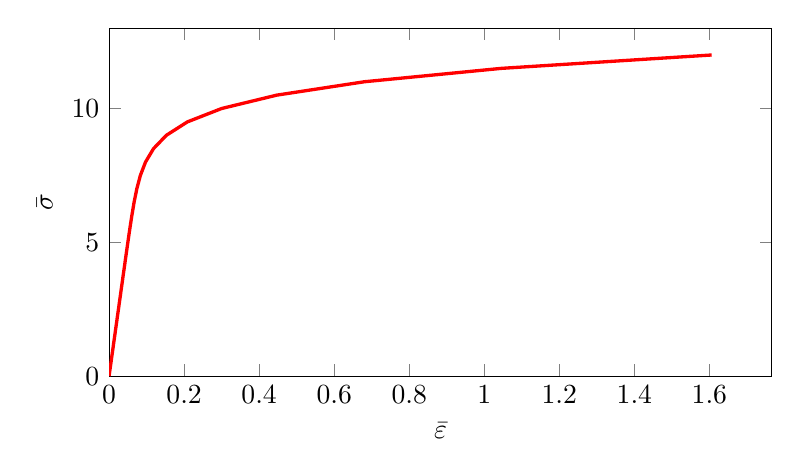
\begin{tikzpicture}
\begin{axis}[
height=6cm,width=10cm,
ymin=0,ymax=13,
xmin=0,
xlabel=$\bar\varepsilon$,
ylabel=$\bar\sigma$,
]
\addplot[domain=0:12,very thick,red](x/100+2*x/100*(x/10)^10,x);
\end{axis}
\end{tikzpicture}
\end{figure}
\subsection{Formulation}
The residual equation is formulated as
\begin{gather}
R=\bar\sigma+\alpha\bar\sigma\left(\dfrac{\bar\sigma}{\bar\sigma^y}\right)^{n-1}-E\bar\varepsilon,
\end{gather}
its derivative with regard to $\bar\sigma$ is
\begin{gather}
\pdfrac{R}{\bar\sigma}=1+n\alpha\left(\dfrac{\bar\sigma}{\bar\sigma^y}\right)^{n-1}.
\end{gather}
Once $\bar\varepsilon$ and $\bar\sigma^y$ are determined, $\bar\sigma$ can be iteratively computed.

For cyclic loads, it is necessary to record the location of reversing point, denoted by $\varepsilon^r$ and $\sigma^r$. Then,
\begin{gather}
\bar\varepsilon=\abs{\varepsilon-\varepsilon^r},\qquad
\bar\sigma=\abs{\sigma-\sigma^r}.
\end{gather}
It simply means $\bar\varepsilon$ and $\bar\sigma$ are the absolute strain and stress measured from the reversing point.

The yield stress is taken as
\begin{gather}
\bar\sigma^y=\sigma^y+\abs{\sigma^r}.
\end{gather}
where $\sigma^y$ is the initial yield stress. This definition is fine for large cycle loads, but not sufficient for small cycle loads. For which, the previous reversing point shall be used, let $\varepsilon^{pr}$ and $\sigma^{pr}$ denote its strain and stress, then for small cycles, $\abs{\sigma^{pr}}>\abs{\sigma^{r}}$,
\begin{gather}
\bar\sigma^y=\abs{\sigma^{pr}-\sigma^{r}}.
\end{gather}

To wrap up,
\begin{gather}
\bar\sigma^y=\left\{
\begin{array}{ll}
\max\left(\sigma^y+\abs{\sigma^r},\abs{\sigma^{pr}-\sigma^{r}}\right),&\text{if~}\sigma^{pr}=0\text{~or~}\abs{\sigma^{pr}}<\abs{\sigma^{r}},\\
\abs{\sigma^{pr}-\sigma^{r}},&\text{otherwise}.
\end{array}\right.
\end{gather}
\subsection{Implementation}
The CPP implementation can be found as follows.
\begin{cppcode}
RambergOsgood::update_trial_status
\end{cppcode}
\section{MPF Steel Model}
The MPF model is a widely used phenomenological model for steel.
It was initially proposed with no hardening.
Later, isotropic hardening was introduced as an enhancement.
\subsection{Theory}
The core of the MPF model is the following parametric equation.
\begin{gather}\label{eq:mpf}
	y=bx+\dfrac{\left(1-b\right)x}{\left(1+|x|^r\right)^{\frac{1}{r}}}.
\end{gather}
The equation is controlled by two parameters, $b$ and $r$.
By varying them, one can plot a series of curves.
\begin{figure}[ht]
	\centering
	\begin{subfigure}[t]{0.48\textwidth}
		\centering
		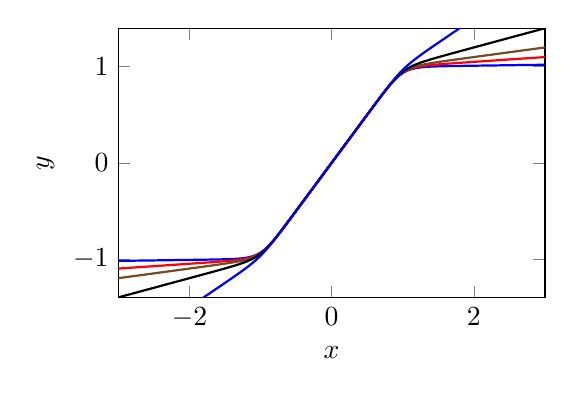
\begin{tikzpicture}
			\begin{axis}[
					height=5cm,width=7cm,
					ymin=-1.4,ymax=1.4,
					xmin=-3,xmax=3,
					xlabel=$x$,
					ylabel=$y$,
				]
				\addplot+[domain=-3:3,thick,samples=100,mark=none]{.01*x+(1-.01)*x*(1+x^10)^(-1/10)};
				\addplot+[domain=-3:3,thick,samples=100,mark=none]{.05*x+(1-.05)*x*(1+x^10)^(-1/10)};
				\addplot+[domain=-3:3,thick,samples=100,mark=none]{.1*x+(1-.1)*x*(1+x^10)^(-1/10)};
				\addplot+[domain=-3:3,thick,samples=100,mark=none]{.2*x+(1-.2)*x*(1+x^10)^(-1/10)};
				\addplot+[domain=-3:3,thick,samples=100,mark=none]{.5*x+(1-.5)*x*(1+x^10)^(-1/10)};
			\end{axis}
		\end{tikzpicture}
		\caption{varying $b$}
	\end{subfigure}\quad
	\begin{subfigure}[t]{0.48\textwidth}
		\centering
		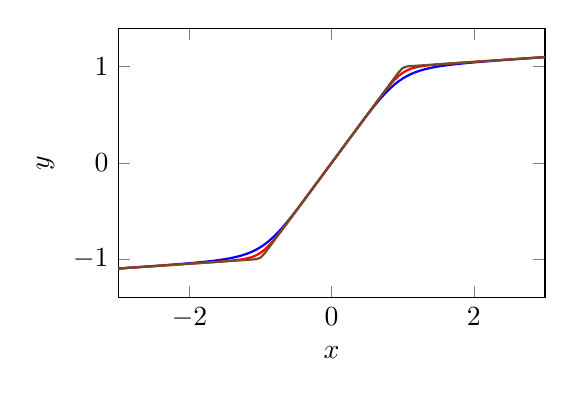
\begin{tikzpicture}
			\begin{axis}[
					height=5cm,width=7cm,
					ymin=-1.4,ymax=1.4,
					xmin=-3,xmax=3,
					xlabel=$x$,
					ylabel=$y$,
				]
				\addplot+[domain=-3:3,thick,samples=100,mark=none]{.05*x+(1-.05)*x*(1+abs(x)^5)^(-1/5)};
				\addplot+[domain=-3:3,thick,samples=100,mark=none]{.05*x+(1-.05)*x*(1+abs(x)^10)^(-1/10)};
				\addplot+[domain=-3:3,thick,samples=100,mark=none]{.05*x+(1-.05)*x*(1+abs(x)^50)^(-1/50)};
			\end{axis}
		\end{tikzpicture}
		\caption{varying $r$}
	\end{subfigure}
\end{figure}
One may observe that \eqsref{eq:mpf} passes through the origin and bends around point $(1,1)$ (or $(-1,-1)$).
Furthermore, parameter $b$ controls the hardening ratio, while $r$ controls the transition from pre-yielding to post-yielding. A sufficiently large $r$ approximates a bilinear model.

One can thus use this equation to construct a constitutive model.
To match the actual Young's modulus, it is possible to define
\begin{gather}\label{eq:mpf_scaled}
	x=\dfrac{\varepsilon}{\varepsilon^y},\qquad
	y=\dfrac{\sigma}{\sigma^y},
\end{gather}
where $\varepsilon^y$ and $\sigma^y$ are the yield strain and stress, respectively.
Such a model asymptotically approaches the bilinear model.
\eqsref{eq:mpf_scaled} alone is not sufficient to describe the cyclic response.
To account for cyclic response, one needs to further introduce the following.
\begin{gather}
	x=\dfrac{\varepsilon-\varepsilon^r}{\varepsilon^y},\qquad
	y=\dfrac{\sigma-\sigma^r}{\sigma^y},
\end{gather}
where $\varepsilon^r$ and $\sigma^r$ are the strain and stress at the load reversing point.
They are updated whenever the load direction changes during the loading process.

One may observe that the MPF model is very similar to the Ramberg--Osgood model.
They adopts the same approach to describe the cyclic response, but with different backbone curves.

Furthermore, $\varepsilon^y$, $\sigma^y$, $r$ and $b$ do not need to be constants.
They can evolve with the loading process, characterized by some measure of plasticity.
In specific, the following can be used.
\begin{itemize}
	\item $\sigma^y$ --- isotropic hardening
	\item $\sigma^y/\varepsilon^y$ --- stiffness degradation
	\item $r$ --- Bauschinger effect
	\item $b$ --- progressive hardening/softening
\end{itemize}

In Filippou's modification,
\begin{gather}
	r=r_0-\dfrac{a_1\zeta}{a_2+\zeta},\qquad
	\dfrac{\sigma^y-\sigma^y_0}{\sigma^y_0}=a_3\left(\dfrac{\varepsilon_{max}}{\varepsilon^y}-a_4\right)\geqslant1,
\end{gather}
where $\zeta$ is difference between previous two reversed points, $\varepsilon_{max}$ is the maximum absolute strain of the whole loading process.
\subsection{Formulation}
\subsection{Implementation}
The CPP implementation can be found as follows.
\begin{cppcode}
MPF::update_trial_status
\end{cppcode}
\section{Bouc--Wen Model}
\subsection{Theory}
The relative resistance can be expressed as a summation of two terms.
\begin{gather}
\dfrac{f}{f_y}=a\dfrac{u}{u_y}+\left(1-a\right)z.
\end{gather}
In which $a$ denotes the hardening ratio.
The field $z$ is an internal variable that does not necessarily possess any physical meaning.
Judging from its form in the above expression, one can infer that $z$ is some sort of relative displacement, similar to $u/u_y$.
It's evolution is governed by the following ODE.
\begin{gather}\label{eq:bouc-wen}
\dot{z}=\dfrac{\dot{u}}{u_y}\left(A-\left(\gamma+\sign{z\dot{u}}\beta\right)\abs{z}^n\right).
\end{gather}
In this incremental form, for a given $\Delta{}u$, using the implicit Euler method, one can obtain
\begin{gather}
R=z-z_n-\dfrac{\Delta{}u}{u_y}\left(A-\left(\gamma+\sign{z\Delta{}u}\beta\right)\abs{z}^n\right).
\end{gather}
Its derivatives are then
\begin{gather}
\pdfrac{R}{u}=\dfrac{A-\left(\gamma+\sign{z\Delta{}u}\beta\right)\abs{z}^n}{u_y},\\
\pdfrac{R}{z}=\dfrac{1}{z}\left(z+\dfrac{\Delta{}u}{u_y}n\left(\gamma+\sign{z\Delta{}u}\beta\right)\abs{z}^n\right).
\end{gather}
Denoting $P=\left(\gamma+\sign{z\Delta{}u}\beta\right)\abs{z}^n$, the tangent stiffness can then be written as
\begin{gather}\label{eq:bouc-wen-stiffness}
\begin{split}
\ddfrac{f}{u}=\pdfrac{f}{u}+\pdfrac{f}{z}\ddfrac{z}{u}&=\pdfrac{f}{u}-\pdfrac{f}{z}\left(\pdfrac{R}{z}\right)^{-1}\pdfrac{R}{u}\\
&=f_y\left(\dfrac{a}{u_y}-\left(1-a\right)\dfrac{zA-zP}{zu_y+\Delta{}unP}\right).
\end{split}
\end{gather}

The Bouc--Wen model \cite{Wen1976} is mainly driven by the ODE \eqsref{eq:bouc-wen}, this makes the formulation extremely simple, to implement such a model, one only needs to solve the ODE using a proper method.
Here we have presented the formulation using the implicit Euler method. Other methods, such as the trapezoidal method, or even multi-step methods, can also be used.
The adoption of various solving method does not actually affect the computation of tangent stiffness.
Once the convergence is achieved, \eqsref{eq:bouc-wen-stiffness} can be used to compute the stiffness.

The Bouc--Wen model has received many criticisms. Since it is a phenomenological model, in which the internal field $z$ has no physical implication, this model may violate thermodynamics.
To alleviate the potential problems, the following constraints are imposed \cite{Ma2004}.
\begin{gather}
A=1,\qquad\gamma+\beta=1.
\end{gather}
\subsection{Formulation}
\subsection{Implementation}
\begin{cppcode}
BoucWen::update_trial_status
\end{cppcode}
\section{General Framework for Hysteresis Models}
\subsection{Theory}
The general framework consists of three main elements:
\begin{enumerate}
\item backbone curve --- compression/tension envelope, \textcolor{blue}{blue} curves in \figref{fig:general_hysteresis}
\item unloading curve --- unload from backbone to the corresponding residual point (with zero stress), \textcolor{green}{green} curves in \figref{fig:general_hysteresis}
\item reloading curve --- loading from residual point to backbone curve on the opposite side, \textcolor{purple}{purple} curves in \figref{fig:general_hysteresis}
\end{enumerate}
Each of those three curves can be either linear/nonlinear or piece-wise linear/nonlinear and may depend on other internal variables.

Accordingly, at least four points are essential to control the response of the model, namely, the tension unloading point, the tension residual point, the compression unloading point, the compression residual point. A schematic illustration is given in \figref{fig:general_hysteresis}. Some complex models may consist of more control points, such as reloading points that connect reloading curves with backbones.
\begin{figure}[ht]
\centering\footnotesize
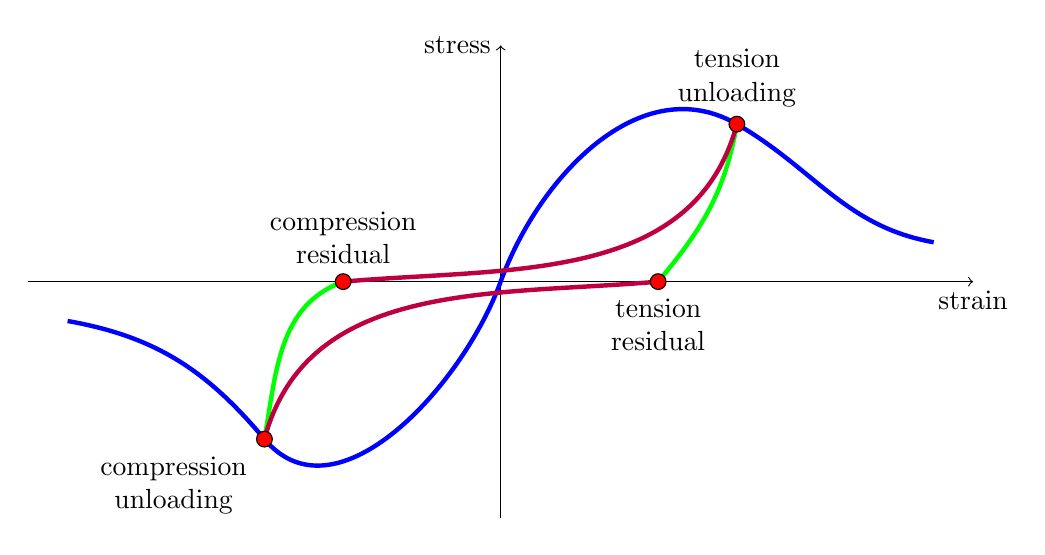
\begin{tikzpicture}
\draw[->](-6,0)--(6,0)node[below]{strain};
\draw[->](0,-3)--(0,3)node[left]{stress};
\coordinate(A)at(0,0);
\coordinate(B)at(3,2);
\coordinate(C)at(5.5,.5);
\coordinate(D)at(2,0);
\draw[ultra thick,blue](A)to[out=70,in=150](B)to[out=-30,in=170](C);
\draw[ultra thick,green](B)to[out=260,in=50](D);
\coordinate(E)at(-3,-2);
\coordinate(F)at(-5.5,-.5);
\coordinate(G)at(-2,0);
\draw[ultra thick,blue](A)to[out=-110,in=-50](E)to[out=130,in=-10](F);
\draw[ultra thick,green](E)to[out=80,in=200](G);
\draw[ultra thick,purple](D)to[out=185,in=75](E)(G)to[out=5,in=-105](B);
\draw[fill=red](B)circle(1mm)node[above=1mm,align=center]{tension\\unloading};
\draw[fill=red](D)circle(1mm)node[below=1mm,align=center]{tension\\residual};
\draw[fill=red](E)circle(1mm)node[below left=1mm,align=center]{compression\\unloading};
\draw[fill=red](G)circle(1mm)node[above=1mm,align=center]{compression\\residual};
\end{tikzpicture}
\caption{schematic illustration a generalised hysteresis model}\label{fig:general_hysteresis}
\end{figure}

With the above definition, it is clear that any given current state $\varepsilon_n$ and $\sigma_n$ shall on one of three curves. With prescribed strain increment $\Delta\varepsilon$, the determination of stress $\sigma_{n+1}$ is equivalent to computing the new point on one of three curves. As the current state $(\varepsilon_n,\sigma_n)$ has to be on one of three curves, it is easy to determine whether $\varepsilon_{n+1}=\varepsilon_n+\Delta\varepsilon$ is on unloading/reloading/backbone curve by simply comparing the magnitudes of $\varepsilon_{n+1}$ and that of unloading/residual strain, which are stored as history variables.

The state determination algorithm can be cast in a branching programming style. In the following procedure, $\varepsilon_{cr}$ is compression residual strain, $\varepsilon_{cu}$ is compression unloading strain, $\varepsilon_{tr}$ is tension residual strain, $\varepsilon_{tu}$ is tension unloading strain.
\begin{breakablealgorithm}
\caption{state determination of general hysteresis model}\label{algo:gen_hys}
\begin{algorithmic}[1]
\State \textbf{Parameter}: necessary model parameters
\State \textbf{Input}: $\varepsilon_{n+1}$, $\varepsilon_n$, $\sigma_n$ and other relevant history variables
\State \textbf{Output}: $E_{n+1}$, $\sigma_{n+1}$ and other relevant history variables
\State get strain values of four control points
\State $\varepsilon_{n+1}=\varepsilon_n+\Delta\varepsilon$
\State determine which curve the new state is on based on the curve the current state is on and the magnitudes of $\varepsilon_{n+1}$, $\varepsilon_{cr}$, $\varepsilon_{cu}$, $\varepsilon_{tr}$,  $\varepsilon_{tu}$
\State call corresponding methods to compute the new state $(\varepsilon_{n+1},\sigma_{n+1})$ based on relevant two control points and history variables, if any
\end{algorithmic}
\end{breakablealgorithm}

\subsection{Implementation}
By using two flags, it is easy to track which curve each point is on.
\begin{cppcode}
	enum class Status { NONE, CBACKBONE, TBACKBONE, CINNER, TINNER };

	Status trial_flag = Status::NONE, current_flag = Status::NONE;
\end{cppcode}

The implementation presented uses a nested structure to simply the procedure. The top level determines whether the new state is on the backbone, if not, the second level determines whether the new state is on the corresponding unloading curve or reloading curve and computes the response accordingly.

For each curve, a universal interface can be provided such that each takes $\varepsilon_{n+1}$ as the input and returns $\sigma_{n+1}$ and $E_{n+1}$ in an array.
\begin{cppcode}
	[[nodiscard]] virtual podarray<double> compute_compression_backbone(double) const = 0;
	[[nodiscard]] virtual podarray<double> compute_tension_backbone(double) const = 0;
	[[nodiscard]] podarray<double> compute_compression_inner(double) const;
	[[nodiscard]] podarray<double> compute_tension_inner(double) const;
\end{cppcode}
The control points can be updated on the demand with some auxiliary methods.
\begin{cppcode}
	[[nodiscard]] virtual podarray<double> compute_compression_initial_reverse() const = 0;
	[[nodiscard]] virtual podarray<double> compute_tension_initial_reverse() const = 0;
	[[nodiscard]] virtual double compute_compression_residual(double, double) const = 0;
	[[nodiscard]] virtual double compute_tension_residual(double, double) const = 0;
\end{cppcode}

The following CPP code snippet shows a working implementation of such a state determination procedure.
\begin{cppcode}
SimpleHysteresis::update_trial_status
\end{cppcode}
\subsubsection{Remarks}
A lot of hysteresis models can be reformulated in the above framework. For example, by fixing residual points to origin, all unloading paths (either linear or nonlinear) converge to origin, which correspond to a class of models that are often called origin--oriented. Alternatively, the reloading curve can be defined in a way so that it always loads back to the peak point on the backbone curve on the opposite side. This is often known as peak--oriented model.

Some complex models suitable for concrete can be formulated accordingly, in which the curves are nonlinear and depend on other internal variables as well. Given that tension response and compression response are independent from each other, some asymmetric models can also be defined.

Noting that the top level branching does not care about history variables, the updating of them are solely handled in the corresponding methods. The presented framework provides a flexible container so that a wide range of models can be defined.

